\documentclass{article}


\relax % Controls
    \newif\ifmarginprooflinks
    	\marginprooflinkstrue
    	% \marginprooflinksfalse

\relax % Bibliography, etc
	\usepackage[american]{babel}
	\usepackage{csquotes}
	\usepackage[backend=biber, style=authoryear]{biblatex}
	\DeclareLanguageMapping{american}{american-apa}
	% \usepackage[backend=biber,style=authoryear,hyperref=true]{biblatex}
	% \addbibresource{refs.bib}
	% \addbibresource{conf.bib}

	\DeclareFieldFormat{citehyperref}{%
	  \DeclareFieldAlias{bibhyperref}{noformat}% Avoid nested links
	  \bibhyperref{#1}}

	\DeclareFieldFormat{textcitehyperref}{%
	  \DeclareFieldAlias{bibhyperref}{noformat}% Avoid nested links
	  \bibhyperref{%
	    #1%
	    \ifbool{cbx:parens}
	      {\bibcloseparen\global\boolfalse{cbx:parens}}
	      {}}}

	\savebibmacro{cite}
	\savebibmacro{textcite}

	\renewbibmacro*{cite}{%
	  \printtext[citehyperref]{%
	    \restorebibmacro{cite}%
	    \usebibmacro{cite}}}

	\renewbibmacro*{textcite}{%
	  \ifboolexpr{
	    ( not test {\iffieldundef{prenote}} and
	      test {\ifnumequal{\value{citecount}}{1}} )
	    or
	    ( not test {\iffieldundef{postnote}} and
	      test {\ifnumequal{\value{citecount}}{\value{citetotal}}} )
	  }
	    {\DeclareFieldAlias{textcitehyperref}{noformat}}
	    {}%
	  \printtext[textcitehyperref]{%
	    \restorebibmacro{textcite}%
	    \usebibmacro{textcite}}}

	\DeclareCiteCommand{\brakcite}
	  {\usebibmacro{prenote}}
	  {\usebibmacro{citeindex}%
	   \printtext[bibhyperref]{[\usebibmacro{cite}]}}
	  {\multicitedelim}
	  {\usebibmacro{postnote}}

\relax % Standard Packages
    \usepackage[dvipsnames]{xcolor}
    % \usepackage[utf8]{inputenc}
    \usepackage{mathtools}
    \usepackage{amssymb}
		\DeclareMathSymbol{\shortminus}{\mathbin}{AMSa}{"39}
    % \usepackage{parskip}
    % \usepackage{algorithm}
    \usepackage{bbm}
	\usepackage{lmodern}
	% \usepackage{times}
    \usepackage{faktor}
    % \usepackage{booktabs}
	% \usepackage[margin=1in]{geometry}
    \usepackage{graphicx}
    \usepackage{scalerel}
    \usepackage{enumitem}
    \usepackage{nicefrac}\let\nf\nicefrac

    % \usepackage{color}
    %\usepackage{stmaryrd}
    \usepackage{hyperref} % Load before theorems...
        \hypersetup{colorlinks=true, linkcolor=blue!75!black, urlcolor=magenta, citecolor=green!50!black}

\usepackage{tikz}
	\usetikzlibrary{positioning,fit,calc, decorations, arrows, shapes, shapes.geometric}
	\usetikzlibrary{cd}

	%%%%%%%%%%%%
	\tikzset{AmpRep/.style={ampersand replacement=\&}}
	\tikzset{center base/.style={baseline={([yshift=-.8ex]current bounding box.center)}}}
	\tikzset{paperfig/.style={center base,scale=0.9, every node/.style={transform shape}}}

	% Node Stylings
	\tikzset{dpadded/.style={rounded corners=2, inner sep=0.7em, draw, outer sep=0.3em, fill={black!50}, fill opacity=0.08, text opacity=1}}
	\tikzset{dpad0/.style={outer sep=0.05em, inner sep=0.3em, draw=gray!75, rounded corners=4, fill=black!08, fill opacity=1, align=center}}
	\tikzset{dpadinline/.style={outer sep=0.05em, inner sep=2.5pt, rounded corners=2.5pt, draw=gray!75, fill=black!08, fill opacity=1, align=center, font=\small}}

 	\tikzset{dpad/.style args={#1}{every matrix/.append style={nodes={dpadded, #1}}}}
	\tikzset{light pad/.style={outer sep=0.2em, inner sep=0.5em, draw=gray!50}}

	\tikzset{arr/.style={draw, ->, thick, shorten <=3pt, shorten >=3pt}}
	\tikzset{arr0/.style={draw, ->, thick, shorten <=0pt, shorten >=0pt}}
	\tikzset{arr1/.style={draw, ->, thick, shorten <=1pt, shorten >=1pt}}
	\tikzset{arr2/.style={draw, ->, thick, shorten <=2pt, shorten >=2pt}}

	\newcommand\cmergearr[5][]{
		\draw[arr, #1, -] (#2) -- (#5) -- (#3);
		\draw[arr, #1, shorten <=0] (#5) -- (#4);
		}
	\newcommand\mergearr[4][]{
		\coordinate (center-#2#3#4) at (barycentric cs:#2=1,#3=1,#4=1.2);
		\cmergearr[#1]{#2}{#3}{#4}{center-#2#3#4}
		}
	\newcommand\cunmergearr[5][]{
		\draw[arr, #1, -, shorten >=0] (#2) -- (#5);
		\draw[arr, #1, shorten <=0] (#5) -- (#3);
		\draw[arr, #1, shorten <=0] (#5) -- (#4);
		}
	\newcommand\unmergearr[4][]{
		\coordinate (center-#2#3#4) at (barycentric cs:#2=1.2,#3=1,#4=1);
		\cunmergearr[#1]{#2}{#3}{#4}{center-#2#3#4}
		}

\usepackage{amsthm,thmtools} % Theorem Macros
	\usepackage[noabbrev,nameinlink,capitalize]{cleveref}
    \theoremstyle{plain}
    \newtheorem{theorem}{Theorem}
	\newtheorem{coro}{Corollary}[theorem]
    \newtheorem{prop}[theorem]{Proposition}
    \newtheorem{conj}[theorem]{Conjecture}
    \newtheorem{claim}{Claim}
    \newtheorem{remark}{Remark}
    \newtheorem{lemma}[theorem]{Lemma}
    \theoremstyle{definition}
    % \newtheorem{defn}{Definition}
    % \declaretheorem[name=Definition]{defn}
    \declaretheorem[name=Definition, qed=$\square$]{defn}
    \declaretheorem[name=Example, qed=$\triangle$]{example}

	\crefname{defn}{Definition}{Definitions}
	\crefname{prop}{Proposition}{Propositions}
    \crefname{issue}{Issue}{Issues}

\relax %%%%%%%%% GENERAL MACROS %%%%%%%%
    \let\Horig\H
	\let\H\relax
	\DeclareMathOperator{\H}{\mathrm{H}} % Entropy
	\DeclareMathOperator{\I}{\mathrm{I}} % Information
	\DeclareMathOperator*{\Ex}{\mathbb{E}} % Expectation
	\DeclareMathOperator*{\EX}{\scalebox{1.5}{$\mathbb{E}$}}

    \newcommand{\mat}[1]{\mathbf{#1}}
    \DeclarePairedDelimiterX{\infdivx}[2]{(}{)}{%
		#1\;\delimsize\|\;#2%
	}
	\newcommand{\thickD}{I\mkern-8muD}
	\newcommand{\kldiv}{\thickD\infdivx}
	\newcommand{\tto}{\rightarrow\mathrel{\mspace{-15mu}}\rightarrow}

	\newcommand{\datadist}[1]{\Pr\nolimits_{#1}}
	% \newcommand{\datadist}[1]{p_\text{data}}

	\makeatletter
	\newcommand{\subalign}[1]{%
	  \vcenter{%
	    \Let@ \restore@math@cr \default@tag
	    \baselineskip\fontdimen10 \scriptfont\tw@
	    \advance\baselineskip\fontdimen12 \scriptfont\tw@
	    \lineskip\thr@@\fontdimen8 \scriptfont\thr@@
	    \lineskiplimit\lineskip
	    \ialign{\hfil$\m@th\scriptstyle##$&$\m@th\scriptstyle{}##$\hfil\crcr
	      #1\crcr
	    }%
	  }%
	}
	\makeatother
	\newcommand\numberthis{\addtocounter{equation}{1}\tag{\theequation}}

\relax %%%%%%%%%   PDG  MACROS   %%%%%%%%
	\newcommand{\ssub}[1]{_{\!_{#1}\!}}
	% \newcommand{\bp}[1][L]{\mat{p}_{\!_{#1}\!}}
	% \newcommand{\bP}[1][L]{\mat{P}_{\!_{#1}\!}}
	\newcommand{\bp}[1][L]{\mat{p}\ssub{#1}}
	\newcommand{\bP}[1][L]{\mat{P}\ssub{#1}}
	\newcommand{\V}{\mathcal V}
	\newcommand{\N}{\mathcal N}
	\newcommand{\Ed}{\mathcal E}

    \newcommand{\balpha}{\boldsymbol\alpha}
    \newcommand{\bbeta}{\boldsymbol\beta}

	\DeclareMathAlphabet{\mathdcal}{U}{dutchcal}{m}{n}
	\DeclareMathAlphabet{\mathbdcal}{U}{dutchcal}{b}{n}
	\newcommand{\dg}[1]{\mathbdcal{#1}}
	\newcommand{\PDGof}[1]{{\dg M}_{#1}}
	\newcommand{\UPDGof}[1]{{\dg N}_{#1}}
	\newcommand\VFE{\mathit{V\mkern-4mu F\mkern-4.5mu E}}

	\newcommand\Inc{\mathit{Inc}}
	\newcommand{\IDef}[1]{\mathit{IDef}_{\!#1}}
	% \newcommand{\ed}[3]{%
	% 	\mathchoice%
	% 	{#2\overset{\smash{\mskip-5mu\raisebox{-3pt}{${#1}$}}}{\xrightarrow{\hphantom{\scriptstyle {#1}}}} #3} %display style
	% 	{#2\overset{\smash{\mskip-5mu\raisebox{-3pt}{$\scriptstyle {#1}$}}}{\xrightarrow{\hphantom{\scriptstyle {#1}}}} #3}% text style
	% 	{#2\overset{\smash{\mskip-5mu\raisebox{-3pt}{$\scriptscriptstyle {#1}$}}}{\xrightarrow{\hphantom{\scriptscriptstyle {#1}}}} #3} %script style
	% 	{#2\overset{\smash{\mskip-5mu\raisebox{-3pt}{$\scriptscriptstyle {#1}$}}}{\xrightarrow{\hphantom{\scriptscriptstyle {#1}}}} #3}} %scriptscriptstyle
	\newcommand{\ed}[3]{#2%
	  \overset{\smash{\mskip-5mu\raisebox{-1pt}{$\scriptscriptstyle
	        #1$}}}{\rightarrow} #3}

    \newcommand{\nhphantom}[2]{\sbox0{\kern-2%
		\nulldelimiterspace$\left.\delimsize#1\vphantom{#2}\right.$}\hspace{-.97\wd0}}
		% \nulldelimiterspace$\left.\delimsize#1%
		% \vrule depth\dp#2 height \ht#2 width0pt\right.$}\hspace{-.97\wd0}}
	\makeatletter
	\newsavebox{\abcmycontentbox}
	\newcommand\DeclareDoubleDelim[5]{
	    \DeclarePairedDelimiterXPP{#1}[1]%
			{% box must be saved in this pre code
				\sbox{\abcmycontentbox}{\ensuremath{##1}}%
			}{#2}{#5}{}%
		    %%% Correct spacing, but doesn't work with externalize.
			% {\nhphantom{#3}{##1}\hspace{1.2pt}\delimsize#3\mathopen{}##1\mathclose{}\delimsize#4\hspace{1.2pt}\nhphantom{#4}{##1}}
			%%% Fast, but wrong spacing.
			% {\nhphantom{#3}{~}\hspace{1.2pt}\delimsize#3\mathopen{}##1\mathclose{}\delimsize#4\hspace{1.2pt}\nhphantom{#4}{~}}
			%%% with savebox.
		    {%
				\nhphantom{#3}{\usebox\abcmycontentbox}%
				\hspace{1.2pt} \delimsize#3%
				\mathopen{}\usebox{\abcmycontentbox}\mathclose{}%
				\delimsize#4\hspace{1.2pt}%
				\nhphantom{#4}{\usebox\abcmycontentbox}%
			}%
	}
	\makeatother
	\DeclareDoubleDelim
		\SD\{\{\}\}
	\DeclareDoubleDelim
		\bbr[[]]
	% \DeclareDoubleDelim
	% 	\aar\langle\langle\rangle\rangle
	\makeatletter
	\newsavebox{\aar@content}
	\newcommand\aar{\@ifstar\aar@one@star\aar@plain}
	\newcommand\aar@one@star{\@ifstar\aar@resize{\aar@plain*}}
	\newcommand\aar@resize[1]{\sbox{\aar@content}{#1}\scaleleftright[3.8ex]
		{\Biggl\langle\!\!\!\!\Biggl\langle}{\usebox{\aar@content}}
		{\Biggr\rangle\!\!\!\!\Biggr\rangle}}
	\DeclareDoubleDelim
		\aar@plain\langle\langle\rangle\rangle
	\makeatother


	% \DeclarePairedDelimiterX{\aar}[1]{\langle}{\rangle}
	% 	{\nhphantom{\langle}{#1}\hspace{1.2pt}\delimsize\langle\mathopen{}#1\mathclose{}\delimsize\rangle\hspace{1.2pt}\nhphantom{\rangle}{#1}}

\relax %%%%% restatables and links
	% \usepackage{xstring} % for expandarg
	\usepackage{xpatch}
	\makeatletter
	\xpatchcmd{\thmt@restatable}% Edit \thmt@restatable
	   {\csname #2\@xa\endcsname\ifx\@nx#1\@nx\else[{#1}]\fi}% Replace this code
	   % {\ifthmt@thisistheone\csname #2\@xa\endcsname\typeout{oiii[#1;#2\@xa;#3;\csname thmt@stored@#3\endcsname]}\ifx\@nx#1\@nx\else[#1]\fi\else\csname #2\@xa\endcsname\fi}% with this code
	   {\ifthmt@thisistheone\csname #2\@xa\endcsname\ifx\@nx#1\@nx\else[{#1}]\fi
	   \else\fi}
	   {}{\typeout{FIRST PATCH TO THM RESTATE FAILED}} % execute on success/failure
	\xpatchcmd{\thmt@restatable}% A second edit to \thmt@restatable
	   {\csname end#2\endcsname}
	   {\ifthmt@thisistheone\csname end#2\endcsname\else\fi}
	   {}{\typeout{FAILED SECOND THMT RESTATE PATCH}}

	% \def\onlyaftercolon#1:#2{#2}
	\newcommand{\recall}[1]{\medskip\par\noindent{\bf \Cref{thmt@@#1}.} \begingroup\em \noindent
	   \expandafter\csname#1\endcsname* \endgroup\par\smallskip}

   	\setlength\marginparwidth{1.55cm}
	\newenvironment{linked}[3][]{%
		\def\linkedproof{#3}%
		\def\linkedtype{#2}%
		% \reversemarginpar
		% \marginpar{%
		% \vspace{1.1em}
		% % \hspace{2em}
		% 	% \raggedleft
		% 	\raggedright
		% 	\hyperref[proof:\linkedproof]{%
		% 	\color{blue!50!white}
		% 	\scaleleftright{$\Big[$}{\,{\small\raggedleft\tt\begin{tabular}{@{}c@{}} proof of \\\linkedtype~\ref*{\linkedtype:\linkedproof}\end{tabular}}\,}{$\Big]$}}
		% 	}%
        % \restatable[#1]{#2}{#2:#3}\label{#2:#3}%
		\ifmarginprooflinks
		\marginpar{%
			% \vspace{-3em}% %% for bottom
			\vspace{1.5em}
			\centering%
			\hyperref[proof:\linkedproof]{%
            % \hyperref[proof:#3]{
			\color{blue!30!white}%
			\scaleleftright{$\Big[$}{\,\mbox{\footnotesize\centering\tt\begin{tabular}{@{}c@{}}
				% proof of \\\,\linkedtype~\ref*{\linkedtype:\linkedproof}
				link to\\[-0.15em]
				proof
			\end{tabular}}\,}{$\Big]$}}~
			}%
		\fi
        \restatable[#1]{#2}{#2:#3}\label{#2:#3}%
        }%
		{\endrestatable%
		}
	\makeatother
		\newcounter{proofcntr}
		\newenvironment{lproof}{\begin{proof}\refstepcounter{proofcntr}}{\end{proof}}

		\usepackage{cancel}
		\newcommand{\Cancel}[2][black]{{\color{#1}\cancel{\color{black}#2}}}

		\usepackage{tcolorbox}
		\tcbuselibrary{most}
		\tcolorboxenvironment{lproof}{
			% fonttitle=\bfseries,
			% top=0.5em,
			enhanced,
			parbox=false,
			boxrule=0pt,
			frame hidden,
			borderline west={4pt}{0pt}{blue!20!black!40!white},
			% coltext={blue!20!black!60!white},
			colback={blue!20!black!05!white},
			sharp corners,
			breakable,
			% bottomsep at break=4cm,
			% enlarge bottom at break by=-4cm,
			% topsep at break=3cm,
			% enlarge top at break by=-3cm
		}
		% \usepackage[framemethod=TikZ]{mdframed}
		% \surroundwithmdframed[ % lproof
		% 	   topline=false,
		% 	   linewidth=3pt,
		% 	   linecolor=gray!20!white,
		% 	   rightline=false,
		% 	   bottomline=false,
		% 	   leftmargin=0pt,
		% 	   % innerleftmargin=5pt,
		% 	   skipabove=\medskipamount,
		% 	   skipbelow=\medskipamount
		% 	]{lproof}
	%oli16: The extra space was because there was extra space in the paragraph, not
	%because this length was too big. By breaking arrays, everything will be better.
	\newcommand{\begthm}[3][]{\begin{#2}[{name=#1},restate=#3,label=#3]}

\relax %TODOs and footnotes
    \newcommand{\TODO}[1][INCOMPLETE]{{\centering\Large\color{red}$\langle$~\texttt{#1}~$\rangle$\par}}
    \newcommand{\dfootnote}[1]{%
        \let\oldthefootnote=\thefootnote%
        % \addtocounter{footnote}{-1}%
		\setcounter{footnote}{999}
        \renewcommand{\thefootnote}{\textdagger}%
        \footnote{#1}%
        \let\thefootnote=\oldthefootnote%
    }
	\newcommand{\dfootnotemark}{
		\footnotemark[999]
	}


% \usepackage[framemethod=TikZ]{mdframed}
% \colorlet{color1}{Emerald}
% \colorlet{color3}{color1>wheel,2,3}
% \colorlet{pinkish}{color3!25!magenta}
\definecolor{brownish}{rgb}{0.5, 0.2, 0.1}
% \newmdenv[roundcorner=5pt, 
%     backgroundcolor=brownish!20!white,
%     % frametitle={$\langle$under construction$\rangle$},
%     frametitle={$\langle$incomplete or buggy$\rangle$},
%     frametitlerule=false,
%     innertopmargin=3pt, frametitlebelowskip=1ex, frametitleaboveskip=1ex,
%     frametitlebackgroundcolor=brownish!40!white,
%     skipabove=1em,skipbelow=1em,
%     frametitlefont={\scshape},leftmargin=-10pt, rightmargin=-10pt]
% 		{wip}
\newtcolorbox{wip}{%
    colback=brownish!20!white,%
    % frametitle={$\langle$under construction$\rangle$},
    title={$\langle$under construction$\rangle$},%
    enhanced jigsaw,
    breakable,
    % frametitlerule=false,
    % innertopmargin=3pt, frametitlebelowskip=1ex, frametitleaboveskip=1ex,
    colframe=brownish!40!white,%
    % skipabove=1em,skipbelow=1em,
    % frametitlefont={\scshape},leftmargin=-10pt, rightmargin=-10pt
}
        
% \tcolorboxenvironment{example}{
\newtcolorbox[use counter=example]{examplex}{
        fonttitle=\bfseries,
        % empty,
        enhanced jigsaw,
        title={Example \thetcbcounter.},
        before=\par\medskip\noindent,
        % top=0.5em,
        % enhanced,
        parbox=false,
        % boxrule=0pt,
        % frame hidden,
        % borderline west={4pt}{0pt}{green!20!black!40!white},
        % coltext={blue!20!black!60!white},
        % colback={blue!20!black!05!white},
        colback=white,
        sharp corners,
        breakable,
        % bottomsep at break=4cm,
        % enlarge bottom at break by=-4cm,
        % topsep at break=3cm,
        % enlarge top at break by=-3cm
    }

\setlength\parskip{1ex}

\newcommand{\CI}{\mathbin{\bot\!\!\!\bot}}
\newcommand{\Pa}{\mathop{\mathbf{Pa}}}

\begin{document}
    
    \subsection*{Two Equivalent Definitions of Mechanism Independence}
    
    \begin{defn}
        Let $f : X_1 \to \Delta Y_1$ and $g : X_2 \to \Delta Y_2$ be mechanisms.
        We say $f$ and $g$ are independent in a joint distribution $\nu(X_1, X_2, Y_1, Y_2)$ iff
        \begin{enumerate}[nosep]
        \item $\nu(Y_1 \mid X_1) = f$,
        \item $\nu(Y_2 \mid X_2) = g$, and
        \item $\displaystyle Y_1 \underset\nu{\CI} Y_2 \mid X_1, X_2$.
            
        \end{enumerate}        
    \end{defn}
    
    \begin{claim}
        Given a function $f : X \to \Delta Y$, we can construct a ``derandomized'' function $\tilde f : X \times U \to Y$,
        such that 
        \begin{enumerate}[label=(\alph*),nosep]
            \item If $u \in U$ is chosen uniformly at random, then
                the resulting distribution $\tilde f(x, u)$ (a probability over $Y$) equals $f(x)$.  Symbolically:
            \[
                \tilde f^\#(x, \mathrm{Unif}(U)) = f(Y|x) \quad\text{for all } x \in X.
            \]
        \end{enumerate}
    \end{claim}   
    % \begin{proof}
    %     \textbf{(Assume X and Y are finite.)}. 
    % \end{proof}
    
    
    \begin{defn}
        Consider $f : X_1 \times U_1 \to Y_1$ and $g : X_2 \times U_2 \to Y_2$. 
        They are independent in $\nu(X_1, X_2, Y_1, Y_2, U_1, U_2)$
        iff $U_1$ and $U_1$ are independent in $\nu$, conditioned on $X_1$ and $X_2$. 
    \end{defn}
    
    
    \begin{prop}
        $f$ and $g$ are 
    \end{prop}
    
    
    \section{Compatibility with a Set of Type-1 Edges}
    \begin{defn}
        A joint distribution $\mu$ is qualitatively compatible (or q-compatible) with a collection of type-1
        edges
        $\Ed 
        %= \{ \ed {L}{X_L}{Y_L} \}%
        %_{L \in \mathrm{Labels}}
        $ iff
        \begin{enumerate}
            % \item for every pair of disjoint subsets of edges $E_1, E_2 \subset \Ed$, 
            % we have that
            % \[
            %     \Tgt E_1 \underset\mu\CI \Tgt E_2 ~\Big|~ \Src E_1 \cup \Src E_2
            % \]
            \item for every pair of distinct edges $e_1, e_2 \in \Ed$, 
            we have that
            \[
                \Tgt e_1 \underset\mu\CI \Tgt e_2 ~\Big|~ \Src e_1 \cup \Src e_2
            \]
        \end{enumerate}
    \end{defn}
    
    \begin{example}
        \begin{enumerate}[label=\textbf{(\alph*)}]
        \item Suppose $\Ed = \{ \ed1{}X, ~ \ed2{}X \}$ consists of just two edges pointing to $X$.
            Since there is only one pair of distinct edges edges,
            $\mu$ is q-compatible with $\Ed$ iff 
            \begin{align*}
                X \underset\mu\CI X \qquad\iff\qquad \mu(X) = \delta_x \text{ for some }x \in \V(X),
            \end{align*}
            since the only way for a random variable to be independent of itself is if it is deterministic.
            
        \item By the same logic, $\mu$ is q-compatible with $\{ \to\! X, ~Y \!\gets \}$ iff
            % $\mu(X,Y) = \mu(X)\mu(Y)$.                
            $X \CI_\mu Y$. 

        \item Generalizing the first example, 
        $\mu$ is q-compatible with 
        $\Ed = \{ \ed1{X\!}{\!Y}, ~ \ed2{X\!}{\!Y} \}$ 
        % $\Ed = [  ] 
        consisting of two parallel edges iff
        \begin{align*}
            Y \underset\mu\CI Y \mid X \qquad
            &\iff\qquad \mu(Y, Y, X) \mu(X) = \mu(Y, X)\mu(Y,X)
            % \\&\iff\qquad \mu(X) = \mu(Y,X) \text{ or } \mu(X,Y) = 0
            \\&\iff\qquad \mu(X,Y) \in \{\mu(X), 0\}
            \\&\iff\qquad\text{the value of $Y$ is fully determined by $X$ in $\mu$}
            \\&\iff\qquad \H_{\mu}(Y|X) = 0            
        \end{align*}
        
        \end{enumerate}
    \end{example}
    
    
    \begin{example}
        Consider $\Ed = \{ \ed 1{}{\!X},~ \ed2{Y\!}{\!X} \}$.
        A distribution $\mu$ is q-compatible with $\Ed$ iff
        \[
            X \underset\mu\CI X \mid Y \quad\iff\quad \text{$X$ is a function of $Y$}
            \quad\iff\quad \H_\mu(X|Y) = 0
        \] 
    \end{example}
    
    \begin{remark}
        From the above, we can see that our definition does not distinguish between the qualitative PDGs
        \vspace{-2ex}
        \[
            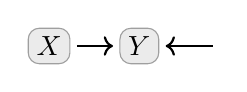
\begin{tikzpicture}[center base]
                \node[dpad0] (X) {$X$};
                \node[dpad0,right=0.6 of X] (Y) {$Y$};
                \draw[arr2] (X) -- (Y);
                \draw[arr2, <-] (Y) -- ++(1, 0);
            \end{tikzpicture}
            \quad~ \text{and}\qquad
            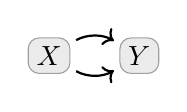
\begin{tikzpicture}[center base]
                \node[dpad0] (X) {$X$};
                \node[dpad0,right=0.6 of X] (Y) {$Y$};
                \draw[arr2] (X) to[bend left] (Y);
                \draw[arr2] (X) to[bend right] (Y);
            \end{tikzpicture}
            ~.
        \]
    \end{remark}
    
    % \begin{example}
    %     A joint distribution $\mu$ is  q-compatible with the edges of a BN iff
    %     \begin{align*}
    % 
    %     \end{align*}
    % \end{example}
    \begin{prop}
        A joint distribution $\mu$ is q-compatible with the edges corresponding to the structure of qualitative BN $\mathcal G$%
            \footnote{that is, the edges of the PDG $\PDGof{\mathcal B}$ for a BN $\mathcal B$}
        iff it satisfies the independencies of $\mathcal G$.
                % {\color{red} False!}
    \end{prop}
    \begin{proof}
        % {\color{red} False!}
        $(\implies)$. Suppose that $\mu$ satisfies the independencies of $\mathcal B$.
        Recall that in a BN structure, there is a 1-1 correspondence between hyper-edges $\Ed$ of $\cal B$ and the variables of $\cal B$. 
        So, let $X,Y$ be two variables of $\cal B$.
        
        To show that $\mu$ is q-compatible with $\Ed$, it suffices to show that 
        \[ X \underset\mu\CI  Y ~\Big|~ \Pa( X) \cup \Pa( Y)
            % \qquad\text{---which we do in the appendix}
            . \]
        % By RaU Thm 4.4.4 (CIRV3), it suffices to show
        % \[ \mat X \underset\mu\CI \mat Y \cup \Pa(\mat Y) ~\Big|~ \Pa(\mat X) \]
        This can be proved by appeal to d-separation. 
        Suppose, for contradiction, that $X$ and $Y$ are not d-separated given $\Pa( X)$ and $\Pa(Y)$,
         % i.e., there are variables $X \in \ X$ and $Y \in \mat Y$ that are d-connected given $\Pa(\mat X)$ and $\Pa(\mat Y)$.
        i.e., they are d-connected.
        By definition, this means that there is an undirected path (of edges of $\cal B$) that (1) cannot include parents of $X$ or $Y$ and (2) can only include head-to-head connections of directed edges $\cdots \to Z\gets \cdots$ at those nodes $Z$ which have a parent of $X$ or $Y$ descendent. 
        
        Now, because this path includes neither any parents of $X$ nor $Y$, the edges at the ends of the path must point inwards; the directions of the first and last edges must be: $X \to \cdots \gets Y$. 
        Such a path must necessarily have a head-to-head connection somewhere;
        %---let's call it $Z$---
        let's call $Z_1$ the node closest to $X$ at which this occurs, and analogously, let's call $Z_2$ the closest such node to $Y$.
        By the criteria for d-separatedness, every such node must have a parent of $X$ or $Y$ as a descendent (which we'll call $W_1$ and $W_2$ respectively, for $Z_1$ and $Z_2$). 
        % Without loss of generality, suppose it's a parent of $X$. 
        But this contradicts the fact that $\cal B$ is an acyclic graph! 
        
        Concretely, it must be the case that $W_1$ is not a parent of $X$ (so it is a parent of $Y$), and $W_2$ is not a parent of $Y$ (so it is a parent of $X$). 
        Because if $W_1$ were a parent of $X$, we would have a directed cycle 
        $W_1 \to X \to\cdots\to Z_1 \to \cdots \to W_1,$ 
        and if $W_2$ were a parent of $Y$, we would analogously have the directed cycle 
        $W_2 \to Y \to\cdots\to Z_2 \to \cdots\to W_2$. 
        But we're still in a bind; the only way to prevent this was to have edges $W_2 \to X$ and $W_1 \to Y$, creating the larger directed cycle
        \[
            W_2 \to X \to\!\cdots\!\to Z_1 \to\!\cdots\!\to W_1 \to Y \to\!\cdots\!\to Z_2 \to\!\cdots\!\to W_2.
        \]
        
        % Suppose that there is an undirected path from some $X \in \mat X$ to some $Y \in \mat Y$. Then

        
                
        $(\impliedby)$.
    \end{proof}
    \begin{remark}
        This is not true if we strengthened qualitative consistency to require independence for \textbf{every} disjoint subset of edges (as opposed to just the singletons as we do now)! Counter-example:
        \begin{center}
        \begin{tikzcd}[column sep=1em,row sep=1.5ex]
            X_1 \to \cdots \ar[r] & Z \ar[d] & \ar[l] \cdots \gets Y \\
            & \vdots \ar[d] & \\
            X_2 & \ar[l] W
        \end{tikzcd}
        \end{center}
        In the above BN, it's not the case that
        \(
            \{X_1, X_2\} \CI_{\cal B} Y ~\big|~ W.
        \)
    \end{remark}
    
    
    \begin{claim}
        A distribution $\mu$ is qualitatively compatible with the edges of an unweighted PDG $\dg N$ iff 
        % $\IDef{\dg N}(\mu) \succeq 0$. 
        the information profile vector
    \end{claim}
    
\end{document}
